\chapter{Whiteboard area detection based on special pattern}
Digital cameras are becoming accessible to average users, more and more people use digital cameras to take images of whiteboards instead of copying manually, thus significantly increasing the productivity. The system we describe in this paper aims at reproducing the whiteboard content as a faithful, yet enhanced and easily controllable, electronic document through the use of a camera. However, images are usually taken from an angle to avoid highlights created by flash, resulting in undesired perspective distortion. They also contain other distracting regions such as walls. The system we have developed uses a series of image processing algorithms. It automatically locates the boundary of a whiteboard. We use special ‘star’ pattern for helping us detecting and for making correct transformation of whiteboard. In the first section we will talk about special pattern based identification of whiteboard. Afterwards, we will discuss about using cascade training algorithms for finding the pattern candidates. Then we will tell about local feature analysis for identification of star pattern and choosing the best quadruples from the candidates set. 
\section{Choosing special pattern for identification}
The first task in broadcasting as a live video streaming of a whiteboard content is to identify the whiteboard itself. The only thing that is interested in the whole image frame is only the rectangle of the whiteboard area. All the other stuff that is apart from the whiteboard can be considered as a noise in each frame. The first assumptions is that we have different types of whiteboards. Not all the types of whiteboards can be detected by well-known edge detection algorithms as: Canny’s algorithm, Sobel’s algorithm, Laplacian algorithm, Prewitt’s algorithm, Roberts’s algorithm \cite{Argyle}. The problem is that whiteboard can be without edges, or you cannot use non whiteboard like surface if you pick the way of finding whiteboard only with detecting edges, etc. Our solution is to use special ‘start’ pattern for identification of four corners of whiteboard. Among different shapes the star pattern is tend to be easy drawn by almost any people. Also in terms of pattern analysis it has a special structure that is less common to be met in an ordinary classroom. In many times star image fits into square. It can give us clear vision of how we should transform rectangular whiteboard matrix to get a frontal view and not a view from some angle.
\section{Using cascade training algorithms for pattern detection}
There are several well-known feature detector algorithms and techniques. The ones that are supported by many ready hands-on tools for image processing is: Haar, local binary patterns (LBP), and histograms of oriented gradients (HOG) \cite{Lienhart}. Haar and LBP features are often used to detect faces because they work well for representing fine-scale textures. The HOG features are often used to detect objects such as people and cars. They are useful for capturing the overall shape of an object. So our decision fall into two feature detectors LBP and Haar. Both cascade classifiers need a positive and negative training data. So we have collected sample of about 600 positive and 1100 negative images. As an image we considered the images of hand-written star shape. You can see some of the sample star images in the Figure \ref{fig:star_images_sample}.
\begin{figure}[h]
    \centering
    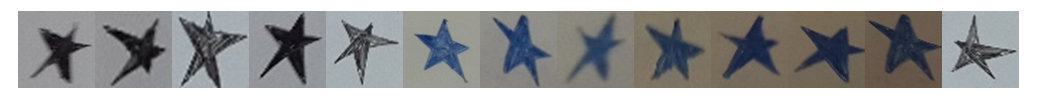
\includegraphics[width=\textwidth]{Figures/star_images_sample}
    \caption{Star image samples}
    \label{fig:star_images_sample}
\end{figure}

In Table \ref{tab:lbp_vs_haar} you can see the main comparison that was enough for deciding totally which feature detector to use in our special case. So we come to decision to use Haar cascading technique which is mainly used for face detection applications currently.

\begin{longtable}[t]{|p{0.30\textwidth}|p{0.35\textwidth}|p{0.15\textwidth}|}
\caption{Comparison table of LBP and Haar}\label{tab:lbp_vs_haar} \\
	\hline
	\textbf{Quality} & \textbf{Local Binary Patterns (LBP)} & \textbf{Haar} \\
	\hline
	\endhead
	Training time 
	& 3-4 hours
	& 15-16 hours\\
	\hline
	Found candidates for a pattern, on average 
	& 50-100
	& 10-15 \\
	\hline
\end{longtable}


While setting up the training parameters we set the false negative rate very high, so that there is a low probability of missing  pattern that are searching. However, the bottlenecks are that we will get extra candidates that are not converging with the pattern. That means we should make an extra checks and analysis. You can see from the Figure 2 that the false negative rate is high enough for not missing needed candidates. In Figure \ref{fig:res_for_training_set} you can see the results of pattern detection for the picture that is used for training set. In the picture there is a lot of star pattern, also some of the non-star patterns. So after the training it correctly identified all the star patterns, however it falsely recognized other regions as a positive sample too. In Figure \ref{fig:res_for_image_from_untrained_set} you can see the results for an image from untrained set. And that it mostly covers all the star image patterns except one, anyway we are assuming that it has a high false negative rate, that we need. Because that one region that the training algorithm couldn't recognize is far from regular hand-drawn star image. Nevertheless, you can see that there is a noises or the candidates for a pattern that are not really looks like a star pattern. One of the main reasons is the quality of image and usage of some image filtering techniques. We will discuss about eliminating those noises in the next section.

\begin{figure}[h]
    \centering
    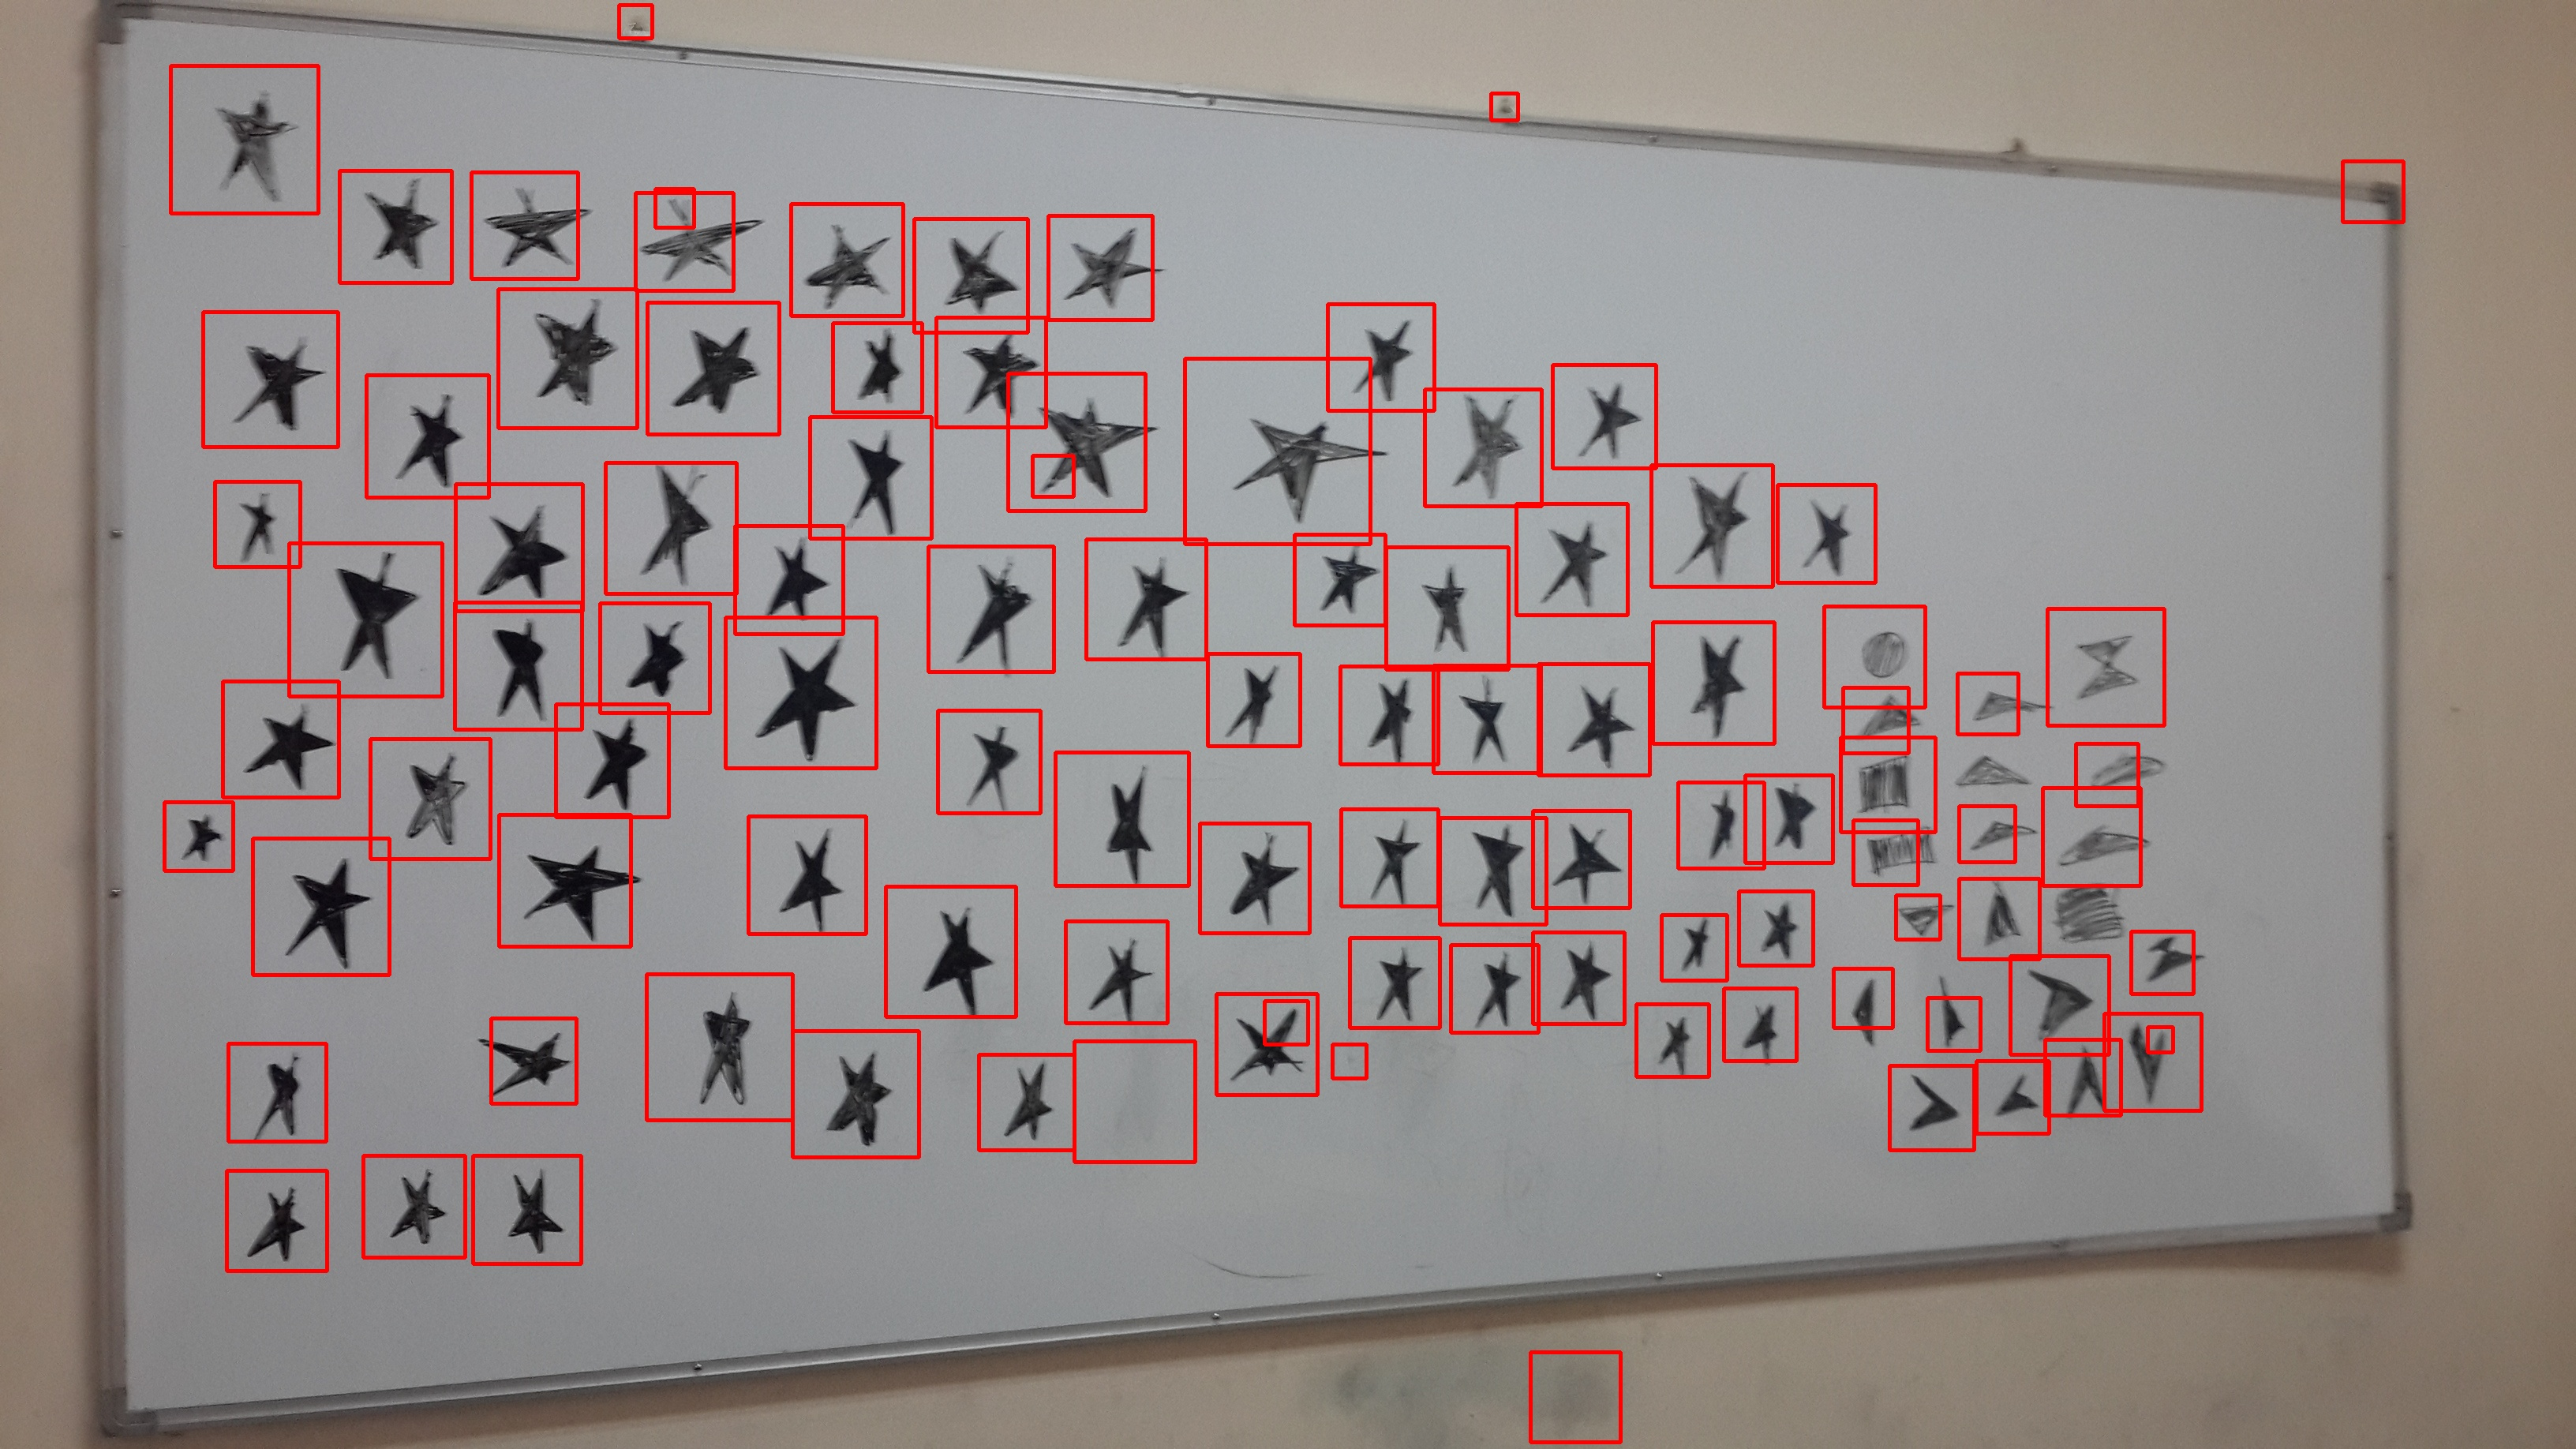
\includegraphics[width=\textwidth]{Figures/res_for_training_set}
    \caption{Results for image from training set}
    \label{fig:res_for_training_set}
\end{figure}

\begin{figure}[h]
    \centering
    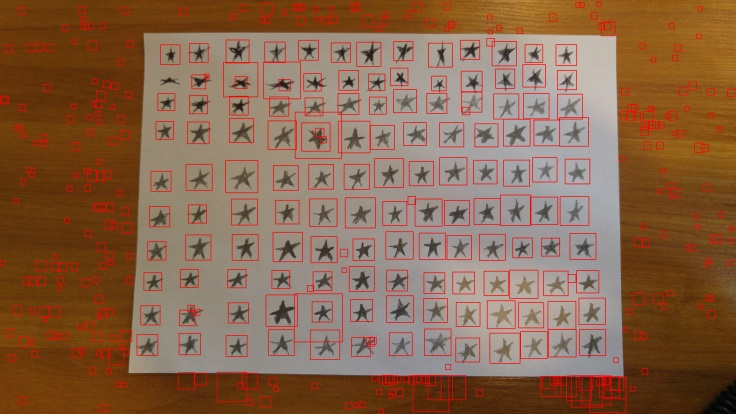
\includegraphics[width=\textwidth]{Figures/res_for_image_from_untrained_set}
    \caption{Results for image from untrained set}
    \label{fig:res_for_image_from_untrained_set}
\end{figure}

\section{Local feature analysis for identification of ‘star’ pattern}
In the previous section we discussed about cascading algorithm which finds the candidates for our pattern from the whole image. It’s false positive rate is set to high and we can see it in practice by the results that it is high enough. So the next process comes to clearing out noises and leaving only star patterns. After some standard filtering and thresholding procedures \cite{Hendeby} we can get binary image for a region. In Figure \ref{fig:transformation_to_binary} you can see results of getting binary images for making the further work easier.

\begin{figure}[h]
    \centering
    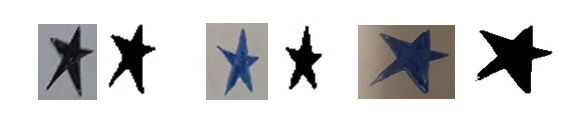
\includegraphics[width=\textwidth]{Figures/transformation_to_binary}
    \caption{Transformation results to binary image }
    \label{fig:transformation_to_binary}
\end{figure}

By using corner and edge detection algorithms \cite{Li} we can find the outer and inner points of the star image. In the Figure \ref{fig:after_corner_detection} we can see the results of applying edge and corner detection algorithms. And the points ‘1’, ‘2’, ‘3’, ‘4’, ‘5’ are considered as an inner points and the points ‘a’, ‘b’, ‘c’, ‘d’, ‘e’ are considered as an outer points of the star image. After making proper matches between inner and outer points we will get different triangles. The cost function in our case is a comparison between perfect star image and the given image. And we will calculate squared error between areas of the triangles of perfect star and given hand-drawn input star. Center of the perfect star will be the mass-center of the given star image that we are processing. And the radius of excircle of the perfect star image is defined by the farthest point from the center. The areas $A, B, C$ that are shown in Figure \ref{fig:perfect_star} are calculated in the following way for the given radius of excircle $R$, with an $S$ being area of pentagon: 

\begin{equation}
    A = R^2 \cdot sin^236 \cdot tg36
\end{equation}
\begin{equation}
    B = A \cdot cos72
\end{equation}
\begin{equation}
    S = \frac{5}{2} \cdot R^2 \cdot sin72
\end{equation}
\begin{equation}
    C = S - 5A - 5B
\end{equation}

And the cost function for the given star image is defined by the following formula:

\begin{equation}
    \sum_{i=1}^{5}(({A_i}' - A)^2 + ({B_i}' - B)^2) + ({C}' - C)^2
\end{equation}

where ${A_1}', {A_2}', \dots {A_5}'$ are triangle areas of type $A$, ${B_1}', {B_2}', \dots {B_5}'$ are triangle areas of type $B$, and ${C}'$ is the area of an inner pentagon.

\begin{figure}[h!]
    \centering
    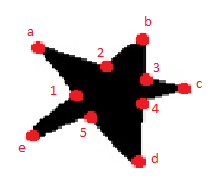
\includegraphics[width={0.35\textwidth}]{Figures/after_corner_detection}
    \caption{Star sample after corner and edge detection}
    \label{fig:after_corner_detection}
\end{figure}

\begin{figure}[h!]
    \centering
    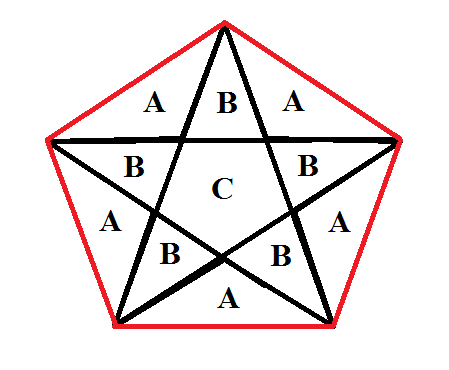
\includegraphics[width={0.35\textwidth}]{Figures/perfect_star}
    \caption{Perfect star pattern with types of triangles and pentagon}
    \label{fig:perfect_star}
\end{figure}

After calculating cost functions for each candidate star pattern we can set some threshold for removing unnecessary noises from the candidate set. Also we can consider all quadruples of stars and choose four star patterns with the lowest cost and compare the figure similarity to the rectangle. By this way we can even cut the candidate set and settle on the four most promising candidates and finish identification process.